\documentclass[12pt, polish, aspectratio = 169]{slides}

\title{Rozprawa Doktorska}
\author{mgr inż. Łukasz Dróżdż}
\subject{Analiza metrologiczna algorytmów dyskretnej transformacji falkowej}
\subtitle{Analiza metrologiczna algorytmów dyskretnej transformacji falkowej}
\institute{Politechnika Śląska, Wydział Elektryczny \\ Katedra Metrologii, Elektroniki i Automatyki}
\keywords{dyskretna transformacja falkowa, cyfrowe przetwarzanie sygnałów, szacowanie niepewności wyniku pomiaru, analiza właściwości metrologicznych toru pomiarowego}

\titlegraphic{
\includegraphics[height = 1cm]{obrazki/polsl_logo}}
\date{30 października 2024}

\begin{document}

\section*{Wstęp do prezentacji oraz plan wystąpienia}

\begin{frame}[plain]
\titlepage
\end{frame}

\begin{frame}{Plan prezentacji}
\tableofcontents
\end{frame}

\newsection{Motywacja pracy}{Przedstawienie motywacji pracy i aktualnego stanu wiedzy}

\begin{frame}{Schemat blokowy toru pomiarowego}
\begin{figure}
\includegraphics[scale = 0.85]{obrazki/schemat_demo}
\caption{Schemat blokowy toru pomiarowego zawierającego w swojej strukturze algorytm transformacji falkowej}
\end{figure}
\begin{itemize}
\item $s(t)$ -- zmienna w czasie wielkość fizyczna.
\item $y(t)$ -- napięciowa reprezentacja wielkości $s(t)$.
\item $x(i)$ -- kolejne próbki wielkości $y(t)$.
\item $\mathbfit{X}(i)$ -- wektor wielkości wyjściowych algorytmu.
\end{itemize}
\end{frame}

\begin{frame}{Algorytm transformacji falkowej}
\begin{equation}
w_{a,b} = \frac{1}{\sqrt{a}} \int _{-\infty} ^{\infty} x \emb{t} \psi \emb{\frac{t-b}{a}} dt \label{eq:cwt}
\end{equation}
\begin{itemize}
\item Umożliwia analizę sygnału $x(t)$ w dziedzinie skala-czas (informacja o czasie).
\item Wykorzystuje funkcję \enquote{falki-matki}, oznaczaną jako $\psi(t)$.
\item Parametr skali $a$ określa wyodrębniany zakres częstotliwości.
\item Parametr $b$ określa przesunięcie falki w czasie (okno pomiarowe).
\item Współczynniki $w_{a,b}$ stanowią wielkości wyjściowe algorytmu.
\end{itemize}
\begin{itemize}
\item[CWT] ciągła transformacja falkowa (w praktyce niemożliwa do realizacji),
\item[DWT] dyskretna transformacja falkowa (dla $a = 2^m$, $b = n2^m$, gdzie $m, n \in \mathbb{N}$),
\item[UFWT] dyskretna transformacja falkowa bez decymacji (bez odrzucania próbek).
\end{itemize}
\end{frame}

\begin{frame}{Obszary zastosowań algorytmu}
\begin{itemize}
\item Przetwarzanie, kompresja oraz analiza obrazów i dźwięków.
\item Pomiary termowizyjne.
\item Redukcja szumu w sygnale pomiarowym.
\item Analiza sygnałów EKG oraz EEG.
\item Analiza przebiegu drgań sejsmicznych.
\item Bezinwazyjna analiza stanu elementów mechanicznych.
\item Algorytmy stratnej kompresji danych.
\item Analiza zwarć wysoko prądowych.
\item Analiza procesów hydrologicznych.
\item Wiele innych zastosowań oraz ciągły ich rozwój.
\end{itemize}
\end{frame}

\begin{frame}{Problem analizy właściwości metrologicznych}
\begin{itemize}
\item Możliwość parametryzacji stosowanego algorytmu:
	\begin{itemize}
	\item zmiana rodzaju stosowanej falki-matki,
	\item zmiana liczby iteracji procesu dekompozycji.
	\end{itemize}
\item Równanie falki matki $\psi(t)$ nie zawsze jest dostępne.
\item Wyprowadzenie odpowiednich zależności jest czasochłonne.
\item Zmiana parametrów stosowanego algorytmu wymusza ponowną analizę.
\item Wymagana jest ekspercka wiedza na temat stosowanej rodziny falek.
\item Metody analityczne są skomplikowane i nie są uniwersalne.
\item Metoda Monte Carlo jest czasochłonna.
\item Brak wskazówek w przewodniku JCGM.
\item Analiza właściwości metrologicznych jest pomijana.
\end{itemize}
\end{frame}

\begin{frame}{Aktualne potrzeby i problemy}
\begin{itemize}
\item Aktualne problemy:
	\begin{itemize}
	\item brak jednolitej metody umożliwiającej wyznaczenie wartości niepewności wielkości wyjściowych algorytmu i opracowanie budżetu niepewności,
	\item dostępne metody są czasochłonne, skomplikowane oraz nie są uniwersalne.
	\end{itemize}
\item Aktualne potrzeby:
	\begin{itemize}
	\item przedstawienie narzędzia umożliwiającego opracowanie budżetu niepewności wielkości wyjściowych algorytmów transformacji falkowej,
	\item zaproponowanie jednolitego modelu błędów, umożliwiającego opis właściwości metrologicznych toru pomiarowego,
	\item zaproponowanie metody umożliwiającej oszacowanie wartości wypadkowej niepewności rozszerzonej dla sporządzonego budżetu niepewności,
	\item proponowane metody muszą być przystępne dla projektanta toru pomiarowego, niebędącego ekspertem w dziedzinie transformacji falkowej.
	\end{itemize}
\end{itemize}
\end{frame}

\newsection{Teza pracy}{Przedstawienie tezy pracy oraz jej najważniejszych założeń}

\begin{frame}{Teza pracy}
\justifying
Stosując przedstawiony model błędów oraz zaproponowaną metodę szacowania wartości wypadkowej niepewności rozszerzonej istnieje możliwość oszacowania wartości niepewności rozszerzonych dla wielkości wyjściowych toru pomiarowego wykorzystującego algorytm dyskretnej transformacji falkowej.

Oszacowanie wartości niepewności rozszerzonych dla omawianych wielkości jest możliwe w trakcie działania systemu pomiarowego, również w przypadku zmiany parametrów pracy tego systemu oraz zmiany parametrów modelu błędów.

Skuteczność zaproponowanej metody oraz dokładność uzyskiwanych wyników zależą od dokładności przyjętych parametrów modelu błędów, przy czym uzyskiwane wyniki są zbieżne z uzyskiwanymi metodą Monte Carlo.
\end{frame}

\begin{frame}{Podsumowanie tezy}
\begin{itemize}
\item Propozycja modelu błędów umożliwiającego opis właściwości metrologicznych torów pomiarowych wykorzystujących analizowane algorytmy oraz przedstawienie ich budżetu niepewności.
\item Propozycja alternatywnej dla metody Monte Carlo metody szacowania wartości wypadkowej niepewności rozszerzonej, która:
	\begin{itemize}
	\item cechuje się niską złożonością obliczeniową i jest możliwa do stosowania w czasie pracy systemu pomiarowego,
	\item daje możliwość zmiany parametrów modelu błędów podczas pracy systemu pomiarowego, zachowując niską złożoność obliczeniową.
	\end{itemize}
\item Wyniki uzyskiwane przy użyciu zaproponowanej metody analizy powinny być zbieżne z wynikami uzyskiwanymi metodą Monte Carlo.
\item Dokładność uzyskiwanych wyników może zależeć od dokładności wyznaczenia parametrów modelu błędu.
\end{itemize}
\end{frame}

\newsection{Model błędów}{Przedstawienie najważniejszych założeń dla zaproponowanego modelu błędów}

\begin{frame}{Model błędów toru pomiarowego}
\begin{figure}
\includegraphics[scale = 0.85]{obrazki/schemat_trans}
\caption{Model błędów pojedynczej wielkości wyjściowej toru pomiarowego}
\end{figure}
\begin{itemize}
\item $s(t)$ -- zmienna w czasie wielkość fizyczna.
\item $y(t)$ -- napięciowa reprezentacja wielkości $s(t)$.
\item $x(i)$ -- kolejne próbki wielkości $y(t)$.
\item $X(i)$ -- wielkość wyjściowa toru pomiarowego.
\item $G_{y}(j\omega)$, $H_{X}(z)$ -- transmitancja części analogowej/cyfrowej.
\item $f_{y}(x)$, $f_{X}(x)$ -- funkcja przetwarzania części analogowej/cyfrowej.
\end{itemize}
\end{frame}

\begin{frame}{Podział sygnałów błędów}
\begin{itemize}
\item Ze względu na charakter realizacji:
	\begin{itemize}
	\item[statyczne] wartość realizacji nie zmienia się w obrębie jednej serii pomiarowej,
	\item[dynamiczne] wartość realizacji zmienia się w obrębie jednej serii pomiarowej oraz można opisać ich przebieg deterministycznie,
	\item[losowe] wartość realizacji zmienia się w obrębie jednej serii pomiarowej oraz nie ma możliwości opisania ich przebiegu deterministycznie.
	\end{itemize}
\item Ze względu na genezę:
	\begin{itemize}
	\item [własne] wprowadzane do sygnału wyjściowego przez analizowany obiekt,
	\item [propagowane] przenoszone z wejścia na wyjście przez analizowany obiekt.
	\end{itemize}
\end{itemize}
\end{frame}

\begin{frame}{Parametry sygnałów błędów}
\begin{itemize}
\item $e(t)$ -- przebieg czasowy sygnału.
\item $E[e(t)]$ -- wartość oczekiwana sygnału.
\item $\sigma^{2}_{e}$ -- wariancja sygnału.
\item $\sigma_{e}$ -- niepewność standardowa.
\item $g(e)$ -- funkcja gęstości prawdopodobieństwa rozkładu wartości realizacji.
\item $U_{e}$ -- niepewność rozszerzona, gdzie $U_{e} = c_{e} \sigma_{e}$.
\item $c_{e}$ -- współczynnik rozszerzenia dla poziomu ufności $1 - \alpha$.
\end{itemize}
\end{frame}

\begin{frame}{Algorytm transformacji falkowej}
\begin{equation}
\begin{bmatrix}
X _{0}   \\
X _{1}   \\
\vdots      \\
X _{M-1}
\end{bmatrix}
=
\begin{bmatrix}
a_{0, 0}   &   a_{0, 1} &   \cdots   &   a_{0, N-1}      \\
a_{1, 0}   &   \ddots   &            &   a_{1, N-1}      \\
\vdots     &            &   \ddots   &   \vdots          \\
a_{M-1, 0} &   \cdots   &   \cdots   &   a_{M-1, N-1}
\end{bmatrix}
\begin{bmatrix}
x _{0}   \\
x _{1}   \\
\vdots      \\
x _{N-1}
\end{bmatrix}
\label{eq:alg_out_mat}
\end{equation}
\begin{itemize}
\item $X_{i}$ -- wielkości wyjściowe algorytmu ($M$ wielkości).
\item $x_{j}$ -- wielkości wejściowe algorytmu ($N$ wielkości).
\item $a_{i,j}$ -- współczynniki macierzy transformacji algorytmu:
	\begin{itemize}
	\item wyznaczane analitycznie, na podstawie właściwości falki-matki,
	\item identyfikowane stosując gotową implementację algorytmu.
	\end{itemize}
\end{itemize}
\end{frame}

\begin{frame}{Właściwości algorytmu transformacji falkowej}
\begin{columns}
\begin{column}{0.5\textwidth}
	\begin{figure}
	\includegraphics[scale = 0.85]{obrazki/dwt_trans}
	\caption{Model właściwości dynamicznych algorytmu transformacji falkowej}
	\end{figure}
\end{column}
\begin{column}{0.5\textwidth}
	\begin{itemize}
	\item $T_{j}(i)$, $S_{j}(i)$ -- detale oraz aproksymacje dla $j$-tej skali.
	\item $x(i)$ -- wielkości wejściowe algorytmu.
	\item $N_{d}$ -- liczba iteracji procesu dekompozycji sygnału wejściowego.
	\item $H_{*}(z)$ -- transmitancja obiektu związanego z wybraną grupą wielkości wyjściowych.
	\end{itemize}
\end{column}
\end{columns}
\end{frame}

\begin{frame}{Właściwości metrologiczne algorytmu}
\begin{itemize}
\item Algorytm przetwarza sygnały błędów obecne w sygnale wejściowym zgodnie z charakterystyką banku filtrów.
\item Rzeczywista implementacja algorytmu wprowadza błędy własne, związane z operacjami arytmetycznymi.
\item Transmitancje obiektów związanych z kolejnymi wielkościami wyjściowymi są ściśle powiązane z macierzą transformacji algorytmu.
\item Konieczne jest określenie:
	\begin{itemize}
	\item parametrów sygnałów błędów na wejściu algorytmu,
	\item parametrów sygnałów błędów własnych algorytmu.
	\end{itemize}
\item Algorytm może tłumić lub wzmacniać sygnały błędów o określonym widmie.
\end{itemize}
\end{frame}

\begin{frame}{Geneza sygnałów błędów własnych}
\begin{enumerate}
\item Wynikające z niedoskonałości transmitancji algorytmu:
	\begin{itemize}
	\item istnieje możliwość deterministycznego opisu przebiegu sygnałów błędów,
	\item sygnały te występują gdy $\tilde{H}_{i}(z) \ne \dot{H}_{i}(z)$,
	\end{itemize}
\item Wynikające z rzeczywistej implementacji algorytmu:
	\begin{itemize}
	\item istnieje możliwość opisu parametrów tych sygnałów w kategoriach probabilistycznych,
	\item występują z uwagi na ograniczone możliwości precyzji zapisu liczb zmiennoprzecinkowych.
	\end{itemize}
\item Wynikające z niedoskonałości wyznaczenia wartości współczynników macierzy transformacji:
	\begin{itemize}
	\item dla błędów numerycznych można zaliczyć je do grupy [2],
	\item w pozostałych przypadkach można zaliczyć je do grupy [1].
	\end{itemize}
\end{enumerate}
\end{frame}

\begin{frame}{Sygnały związane z operacjami numerycznymi}
\begin{figure}
\includegraphics[scale = 0.85]{obrazki/dwt_rerror_coif5_32_pl}
\caption{Zależność wariancji sygnału błędu własnego zaokrągleń od parametrów algorytmu (falka \enquote{coif5}, słowa o długości~\qty{32}{\bitOw})}
\end{figure}
\end{frame}

\begin{frame}{Sygnały związane z operacjami numerycznymi}
\begin{figure}
\includegraphics[scale = 0.85]{obrazki/rerror_db2_2_128_32_pl}
\caption{Zależność wariancji sygnału błędu zaokrągleń od zakresu wartości wielkości wejściowych (falka \enquote{db2}, 2 iteracje dekompozycji, słowa o długości~\qty{32}{\bitOw})}
\end{figure}
\end{frame}

\begin{frame}{Parametry sygnałów błędów własnych}
\begin{columns}
\begin{column}{0.6\textwidth}
	\begin{equation}
	e_{X_{j}}\emb{i} = \tilde{X}_{j}\emb{i} - \dot{X}_{j}\emb{i} \label{eq:dwt_round_error}
	\end{equation}
	\begin{figure}
	\includegraphics[scale = 0.85]{obrazki/schemat_dwt_ew_min}
	\caption{Proces identyfikacji parametrów sygnałów błędów własnych}
	\end{figure}
\end{column}
\begin{column}{0.4\textwidth}
	\begin{itemize}
	\item Parametry sygnału $e_{X_{j}}(i)$ wyznaczane są stosując rzeczywistą implementacje algorytmu.
	\item Sygnały błędów wielkości wejściowych $x(i)$ nie występują.
	\item Parametry sygnału wejściowego $x(i)$ muszą być zbliżone do rzeczywistych.
	\end{itemize}
\end{column}
\end{columns}
\end{frame}

\newsection{Niepewność rozszerzona}{Omówienie stosowanej w pracy metody wyznaczania wartości wypadkowej niepewności rozszerzonej oraz sposobu jej aplikacji}

\begin{frame}{Miara niepewności rozszerzonej}
\begin{columns}
\begin{column}{0.5\textwidth}
	\begin{figure}
	\includegraphics[scale = 0.85]{obrazki/hist_test}
	\caption{Graficzna interpretacja miary niepewności rozszerzonej}
	\end{figure}
\end{column}
\begin{column}{0.5\textwidth}
	\begin{equation}
	P \emb{\left|\hat{e} \emb{t}\right| \le U} = \gamma \label{eq:unc_definition}
	\end{equation}
	\begin{itemize}
	\item Wyznaczana dla wybranego poziomu ufności $\gamma = 1 - \alpha$.
	\item Dostarcza więcej informacji, niż niepewność standardowa.
	\item Wyznaczenie wartości wypadkowej niepewności rozszerzonej może być skomplikowane.
	\end{itemize}
\end{column}
\end{columns}
\end{frame}

\begin{frame}{Wypadkowa niepewność rozszerzona}
\begin{itemize}
\item Analizowana wielkość zakłócona wieloma sygnałami błędów.
\item Rozważane przypadki:
	\begin{itemize}
	\item warunki centralnego twierdzenia granicznego są spełnione,
	\item warunki centralnego twierdzenia granicznego nie są spełnione,
	\item parametry oraz liczba sygnałów błędów mogą się zmieniać.
	\end{itemize}
\item Właściwości algorytmu transformacji falkowej:
	\begin{itemize}
	\item wzmocnia/tłumi sygnały błędów o określonym widmie,
	\item wiele grup wielkości wyjściowych.
	\end{itemize}
\item Problemy:
	\begin{itemize}
	\item metoda Monte Carlo jest skuteczna, jednak bardzo czasochłonna,
	\item metody analityczne są skomplikowane (operacja splotu).
	\end{itemize}
\end{itemize}
\end{frame}

\begin{frame}{Metoda redukcyjnej arytmetyki interwałowej}
\begin{equation}
U_{\Sigma} = \sqrt{
\begin{bmatrix}
U_{0} \\ U_{1} \\ \vdots \\ U_{N-1}
\end{bmatrix}^{T}
\begin{bmatrix}
1         & h_{0,1} & \cdots & h_{0,N-1} \\
h_{1,0}   & 1       &        & h_{1,N-1} \\
\vdots    &         & \ddots & \vdots    \\
h_{N-1,0} & \cdots  & \cdots & 1
\end{bmatrix}
\begin{bmatrix}
U_{0} \\ U_{1} \\ \vdots \\ U_{N-1}
\end{bmatrix}}
\label{eq:unc_matrix}
\end{equation}
\begin{itemize}
\item $h_{i,j} = h_{j,i}$ -- współczynnik koherencji dla pary sygnałów $e_{i}(t)$ oraz $e_{j}(t)$, gdzie $e_{\Sigma}(t) = e_{0}(t) + \hdots + e_{N-1}(t)$, wyznaczane:
	\begin{itemize}
	\item stosując metodę analityczną lub symulacyjną -- proces czasochłonny,
	\item szacując ich wartości -- wyniki mogą być niedokładne,
	\end{itemize}
\item Wartość współczynnika koherencji zależy od parametrów wszystkich analizowanych sygnałów.
\end{itemize}
\end{frame}

\begin{frame}{Aplikacja omawianej metody}
\begin{itemize}
\item Wartości współczynników kształtu wyznaczane na podstawie równania:
\begin{equation}
s_{a,b} = s_{b,a} = \frac{U_{a,b}^{2} - U_{a}^{2} - U_{b}^{2}}{2 U_{a} U_{b}} = \frac{U^{2}}{2 U_{a,b}} - 1 \label{eq:unc_shapertwo}
\end{equation}
\item Korekta wynikająca z centralnego twierdzenia granicznego:
\begin{equation}
k_{i,j} = k_{j,i} = \frac{U_{i}^{2} + U_{j}^{2}}{\sum _{k = 0} ^{N-1} U_{k}^{2}} \label{eq:unc_cohercorrb}
\end{equation}
\item Korekta wynikająca z dysproporcji wartości niepewności rozszerzonych:
\begin{equation}
p_{a,b} = p_{b,a} = \sqrt{\frac{\min \emb{U_{a}, U_{b}}}{\max \emb{U_{a}, U_{b}}}} \label{eq:unc_cohercorra}
\end{equation}
\end{itemize}
\end{frame}

\begin{frame}{Aplikacja omawianej metody}
\begin{itemize}
\item Wartości współczynników koherencji szacowane zgodnie z równaniem:
\begin{equation}
h_{i,j} = h_{j,i} = s_{i,j} p_{i,j} k_{i,j} = s_{i,j} \sqrt{\frac{\min \emb{U_{i}, U_{j}}}{\max \emb{U_{i}, U_{j}}}} \left( \frac{U_{i}^{2} + U_{j}^{2}}{\sum _{k = 0} ^{N-1} U_{k}^{2}} \right) \label{eq:unc_coher}
\end{equation}
\item W celu aplikacji metody należy:
	\begin{itemize}
	\item wyznaczyć wartości współczynników kształtu -- operacja jednorazowa,
	\item skorygować wartości współczynników kształtu dla obecnych parametrów,
	\item zastosować równanie \eqref{eq:unc_matrix} dla uzyskanych wartości.
	\end{itemize}
\item Najistotniejsze cechy metody:
	\begin{itemize}
	\item niska złożoność obliczeniowa -- możliwość stosowania w czasie rzeczywistym,
	\item możliwość zmiany liczby oraz parametrów sygnałów błędów,
	\item względny błąd oszacowania wartości $U_{\Sigma}$ mieszczący się w przedziale \qty{\pm 5}{\percent}.
	\end{itemize}
\end{itemize}
\end{frame}

\newsection{Weryfikacja tezy}{Przedstawienie najważniejszych wyników badań, weryfikujących tezę pracy}

\begin{frame}{Weryfikacja założeń przedstawionych w tezie}
\begin{itemize}
\item Metoda szacowania wartości wypadkowej niepewności rozszerzonej:
	\begin{itemize}
	\item badania symulacyjne przeprowadzone metodą Monte Carlo,
	\item zmienna liczba oraz zmienne parametry sygnałów błędów.
	\end{itemize}
\item Zaproponowany w pracy model błędów:
	\begin{itemize}
	\item symulacyjna weryfikacja przedstawionych zależności dla przykładowego toru pomiarowego metodą Monte Carlo,
	\item pomiarowa weryfikacja przedstawionych zależności dla zbudowanego na potrzeby pracy toru pomiarowego.
	\end{itemize}
\end{itemize}
\end{frame}

\begin{frame}{Wartość wypadkowej niepewności rozszerzonej}
\begin{figure}
\includegraphics[scale = 0.85]{obrazki/hist_rederr_all_2_5_1_20}
\caption{Względny błąd oszacowania wartości wypadkowej niepewności rozszerzonej \textbf{a)}~stosując proponowaną metodę, \textbf{b)}~stosując oryginalną metodę (bez korekty), \textbf{c)}~stosując przewodnik JCGM, $N \in \interval{2}{5}$, $U_{i} \in \interval{1}{20}$, $1-\alpha = \qty{95}{\percent}$}
\end{figure}
\end{frame}

\begin{frame}{Eksperyment symulacyjny}
\begin{figure}
\includegraphics[scale = 0.85]{obrazki/schemat_symul}
\caption{Schemat blokowy toru pomiarowego będącego obiektem eksperymentu symulacyjnego}
\end{figure}
\begin{itemize}
\item $s(t)$ -- zmienna w czasie wielkość fizyczna.
\item $y_{*}(t)$ -- napięciowa reprezentacja wielkości $s(t)$.
\item $x_{*}(i)$ -- dyskretne próbki napięcia reprezentującego wielkość $s(t)$.
\item $\mathbfit{X}(k)$ -- wielkości wyjściowe dla $k$-tej realizacji pomiaru.
\end{itemize}
\end{frame}

\begin{frame}{Założenia eksperymentu symulacyjnego}
\begin{itemize}
\item Przetwarzana wielkość $s(t)$ o przebiegu poliharmonicznym, zakłócona addytywnym szumem białym o stałej widmowej gęstości mocy.
\item Nieidealne właściwości dynamiczne wzmacniacza oraz przetwornika pomiarowego (inercja pierwszego rzędu).
\item Dryft zera wzmacniacza oraz przetwornika zależne liniowo od wolnozmiennej temperatury otoczenia (skorelowane sygnały błędów).
\item Nieidealna charakterystyka statyczna stosowanego wzmacniacza (nieliniowość charakterystyki statycznej).
\item Algorytm transformacji falkowej wprowadza błąd własny wynikający z operacji arytmetycznych (transmitancja algorytmu idealna).
\item Przetwarzanie A/C obarczone błędem kwantowania.
\end{itemize}
\end{frame}

\begin{frame}{Wyniki eksperymentu symulacyjnego}
\begin{table}
\small\caption{Zestawienie wyników eksperymentu symulacyjnego \textbf{a)}~stosując proponowaną metodę, \textbf{b)}~stosując oryginalną metodę (bez korekty), \textbf{c)}~stosując przewodnik JCGM, \textbf{s)}~stosując symulację metodą Monte Carlo (średnia dotyczy wszystkich wielkości)}
\begin{tabular}[c]{| c *{4}{|S[table-format = 3.3]} *{3}{|S[table-format = +1.2]} |} \hline
\multirow{2}{*}{\textbf{Wielkość}} & \multicolumn{4}{c|}{\textbf{Niepewność, mV}} & \multicolumn{3}{c|}{\textbf{Błąd, \%}} \\ \cline{2-8}
          & $U_{c}$ & $U_{a}$ & $U_{b}$ & $U_{s}$ & $\delta_{c}$ & $\delta_{a}$ & $\delta_{b}$ \\ \hline
$S_{2,0}$ & 75.01 & 74.10 & 77.32 & 72.87 & +2.94 & +1.69 & +6.11 \\ \hline
$T_{2,0}$ & 57.29 & 55.91 & 57.58 & 53.89 & +6.31 & +3.75 & +6.85 \\ \hline
$T_{1,0}$ & 47.31 & 43.37 & 46.09 & 43.76 & +8.11 & -0.89 & +5.32 \\ \hline
$T_{1,3}$ & 44.79 & 43.39 & 45.43 & 43.17 & +3.75 & +0.51 & +5.24 \\ \hline
\hline\multicolumn{5}{|c|}{Średnia wartości bezwzględnych wielkości $\delta_{*}$} & 5.77 & 1.48 & 6.13 \\ \hline
\end{tabular}
\end{table}
\end{frame}

\begin{frame}{Eksperyment pomiarowy}
\begin{figure}
\includegraphics[scale = 0.85]{obrazki/schemat_real}
\caption{Schemat blokowy prototypu toru pomiarowego}
\end{figure}
\begin{itemize}
\item $s(t)$ -- zmienne w czasie napięcie wejściowe (RIGOL DG1011).
\item $x(i)$ -- wielkości wejściowe algorytmu transformacji falkowej.
\item $\mathbfit{X}(j)$ -- wielkości wyjściowe dla $j$-tej realizacji pomiaru.
\end{itemize}
\end{frame}

\begin{frame}{Aplikacja zaproponowanej metody analizy}
\begin{enumerate}
\item Określenie, w jaki sposób fragmenty propagują sygnały błędów.
\item Identyfikacja źródeł sygnałów błędów własnych:
	\begin{itemize}
	\item zawartych w sygnale $s(t)$ (parametrów generatora),
	\item wzmacniacza (właściwości statyczne i dynamiczne),
	\item przetwornika A/C (kwantowanie, dynamika układu P/P),
	\item algorytmu transformacji falkowej (operacje zaokrągleń).
	\end{itemize}
\item Identyfikacja parametrów modelu błędów:
	\begin{itemize}
	\item określenie wariancji, wartości oczekiwanej oraz niepewności rozszerzonej,
	\item określenie charakteru realizacji oraz widma sygnałów błędów,
	\item określenie parametrów rozkładu realizacji sygnałów błędów,
	\item określenie korelacji analizowanych sygnałów błędów.
	\end{itemize}
\item Aplikacja zaproponowanej metody szacowania wartości wypadkowej niepewności rozszerzonej.
\end{enumerate}
\end{frame}

\begin{frame}{Identyfikacja żródeł błędów}
\begin{itemize}
\item Wzmacniacz operacyjny w konfiguracji nieodwracającej:
	\begin{itemize}
	\item niedoskonała dynamika obiektu -- $\tilde{K}_{y}(\omega) \cong \dot{K}_{y}(\omega)$, $\tilde{\varphi}_{y}(\omega) \ne \dot{\varphi}_{y}(\omega)$,
	\item niedoskonała statyka obiektu -- przesunięcie charakterystyki, nieliniowość charakterystyki,
	\item inne czynniki - szum na wyjściu, źródło zasilania, zmienna temperatura.
	\end{itemize}
\item Przetwornik A/C oraz układ P/P:
	\begin{itemize}
	\item niedoskonała dynamika obiektu -- $\tilde{K}_{c}(\omega) \cong \dot{K}_{c}(\omega)$, $\tilde{\varphi}_{c}(\omega) \ne \dot{\varphi}_{c}(\omega)$,
	\item niedoskonała statyka obiektu -- błąd wzmocnienia, błędy nieliniowości, błąd przesunięcia zera,
	\item inne czynniki - źródło napięcia referencyjnego, zmienna temperatura.
	\end{itemize}
\end{itemize}
\end{frame}

\begin{frame}{Identyfikacja żródeł błędów}
\begin{itemize}
\item Algorytm transformacji falkowej:
	\begin{itemize}
	\item dokładność wyznaczenia wartości współczynników macierzy transformacji,
	\item operacje arytmetyczne (FPU, instrukcje DSP, słowo~\qty{32}{\bitOwe}).
	\end{itemize}
\item Generator (RIGOL DG1011):
	\begin{itemize}
	\item rozdzielczość przetwornika C/A,
	\item częstotliwość próbek napięcia na wyjściu,
	\item błąd amplitudy oraz składowej stałej,
	\item zniekształcenia harmoniczne,
	\item nieliniowość przetwornika C/A,
	\item zjawisko \enquote{jitter}.
	\end{itemize}
\end{itemize}
\end{frame}

\begin{frame}{Identyfikacja parametrów modelu błędów}
\begin{itemize}
\item Właściwości statyczne toru pomiarowego:
	\begin{itemize}
	\item zastosowanie kalibratora DC (FLUKE 5700A),
	\item badania wykonano dla wielkości $x(i)$,
	\item eksperymenty wykonywano dla stałych warunków otoczenia.
	\end{itemize}
\item Właściwości dynamiczne toru pomiarowego:
	\begin{itemize}
	\item pomiar charakterystyki dynamicznej wzmacniacza (oscyloskop RIGOL DS5062MA oraz generator RIGOL DG1011),
	\item model dynamiczny pierwszego rzędu dla układu P/P (parametry na podstawie dokumentacji układu).
	\end{itemize}
\end{itemize}
\end{frame}

\begin{frame}{Identyfikacja parametrów modelu błędów}
\begin{itemize}
\item Błędy własne algorytmu transformacji falkowej:
	\begin{itemize}
	\item parametry wyznaczono zgodnie z zaproponowaną w pracy metodą,
	\item założono, że transmitancja algorytmu jest idealna,
	\item udział sygnałów błędów własnych okazał się pomijalnie mały.
	\end{itemize}
\item Właściwości generatora przebiegów arbitralnych:
	\begin{itemize}
	\item dokładne badania nie zostały przeprowadzone,
	\item parametry oszacowano na podstawie dokumentacji urządzenia,
	\item opcjonalnie stosowano dodatkowy multimetr (Agilent 3458A).
	\end{itemize}
\end{itemize}
\end{frame}

\begin{frame}{Budżet niepewności wielkości $x(i)$}
\begin{itemize}
\item Niezależne od sygnału $s(t)$:
	\begin{enumerate}
	\item $U_{x,rw} = \qty{0.38}{mV}$ -- właściwości statyczne, rozkład normalny.
	\end{enumerate}
\item Dla monoharmonicznego sygnału $s(t)$:
	\begin{enumerate}
	\item $U_{x,rp}$ -- zniekształcenia harmoniczne generatora, rozkład normalny,
	\item $U_{x,dp}$ -- wypadkowy błąd dynamiczny, rozkład dwumodalny,
	\item $U_{x,sp}$ -- wypadkowy błąd statyczny, rozkład jednostajny.
	\end{enumerate}
\item Dla poliharmonicznego sygnału $s(t)$:
	\begin{enumerate}
	\item $U_{x,rp}$ -- nieliniowość generatora, rozkład jednostajny,
	\item $U_{x,dp}$ -- wypadkowy błąd dynamiczny, splot rozkładów dwumodalnych,
	\item $U_{x,sp}$ -- wypadkowy błąd statyczny, rozkład jednostajny.
	\end{enumerate}
\end{itemize}
\end{frame}

\begin{frame}{Weryfikacja wartości niepewności wielkości $x(i)$}
\begin{table}[p]
\small\caption{Zmierzone oraz oszacowane wartości wypadkowej niepewności rozszerzonej wielkości $x(i)$ (znane parametry sygnału $s(t)$, średnia dla całego eksperymentu)}
\begin{tabular}[c]{| c *{2}{|S[table-format = 4.3]} *{2}{|S[table-format = 4.4]} | S[table-format = +2.2] |} \hline
\multirow{2}{*}{\textbf{$f_{s,o}$, Hz}} & \multicolumn{2}{c|}{\textbf{Wariancja, \micro V}} & \multicolumn{2}{c|}{\textbf{Niepewność, mV}} & \textbf{Błąd, \%} \\ \cline{2-6}
& $\sigma_{c}^{2}$ & $\sigma_{m}^{2}$ & $U_{c}$ & $U_{m}$ & $\delta_{c}$ \\ \hline
600     &       0.59    &       0.44    &       1.24    &       1.16    &       +6.74    \\ \hline
4000    &       24.71   &       20.51   &       7.06    &       6.57    &       +7.48    \\ \hline
8000    &       104.47  &       105.94  &       14.44   &       14.61   &       -1.14    \\ \hline
14000   &       347.53  &       337.12  &       26.31   &       25.84   &       +1.81    \\ \hline
21000   &       857.76  &       775.38  &       41.31   &       39.16   &       +5.49    \\ \hline
\hline\multicolumn{5}{|c|}{Średnia wartości bezwzględnych wielkości $\delta_{*}$} & 5.21 \\ \hline
\end{tabular}
\end{table}
\end{frame}

\begin{frame}{Weryfikacja wartości niepewności wielkości $X_{24}(i)$}
\begin{table}[p]
\small\caption{Zmierzone oraz oszacowane wartości wypadkowej niepewności rozszerzonej wielkości $X_{24}(i)$ (znane parametry sygnału $s(t)$, średnia dla całego eksperymentu)}
\begin{tabular}[c]{| c *{2}{|S[table-format = 4.3]} *{2}{|S[table-format = 4.4]} | S[table-format = +2.2] |} \hline
\multirow{2}{*}{\textbf{$f_{s,o}$, Hz}} & \multicolumn{2}{c|}{\textbf{Wariancja, \micro V}} & \multicolumn{2}{c|}{\textbf{Niepewność, mV}} & \textbf{Błąd, \%} \\ \cline{2-6}
& $\sigma_{c}^{2}$ & $\sigma_{m}^{2}$ & $U_{c}$ & $U_{m}$ & $\delta_{c}$ \\ \hline
600     &       0.51    &       0.48    &       1.39    &       1.37    &       +1.90     \\ \hline
4000    &       224.98  &       186.66  &       21.28   &       19.68   &       +8.12     \\ \hline
8000    &       920.05  &       932.81  &       42.85   &       43.28   &       -0.97     \\ \hline
14000   &       1.07    &       1.88    &       1.96    &       2.73    &       -28.29    \\ \hline
21000   &       2.19    &       32.09   &       2.57    &       8.75    &       -70.59    \\ \hline
\hline\multicolumn{5}{|c|}{Średnia wartości bezwzględnych wielkości $\delta_{*}$} & 12.69 \\ \hline
\end{tabular}
\end{table}
\end{frame}

\begin{frame}{Weryfikacja przyczyny rozbieżności wartości $U_{X_{24},\Sigma}$}
\begin{figure}
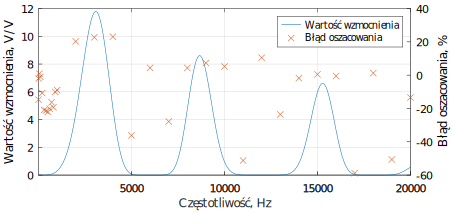
\includegraphics[scale = 0.85]{obrazki/mono_freqcomp}
\caption{Błąd oszacowania wartości niepewności rozszerzonej dla wielkości $X_{24}(i)$}
\end{figure}
\end{frame}

\newsection{Podsumowanie}{Przedstawienie najważniejszych wniosków płynących z pracy}

\begin{frame}{Najważniejsze osiągnięcia pracy}
\begin{itemize}
\item Zaproponowanie jednolitego modelu błędów, opisującego właściwości toru pomiarowego, zarówno części cyfrowej oraz analogowej.
\item Przedstawienie algorytmu transformacji falkowej w postaci macierzowej wraz z metodami identyfikacji wartości współczynników macierzy transformacji.
\item Wskazanie, w jaki sposób algorytm transformacji falkowej przetwarza sygnały błędów z wejścia na wyjście.
\item Opis sygnałów błędów własnych algorytmu transformacji falkowej oraz sposobu identyfikacji ich parametrów.
\item Zaproponowanie przystępnej w aplikacji metody szacowania wartości wypadkowej niepewności rozszerzonej, możliwej do stosowania w czasie rzeczywistym dla zmiennych parametrów modelu błędów.
\item Symulacyjna oraz pomiarowa weryfikacja przedstawionych w pracy zależności oraz wskazanie przykładu aplikacji proponowanej metody analizy.
\end{itemize}
\end{frame}

\begin{frame}{Wnioski}
\begin{itemize}
\item Zaproponowany model błędów jest zasadny w przypadku analizy torów pomiarowych wykorzystujących algorytmy transformacji falkowej.
\item Zaproponowana metoda szacowania wartości wypadkowej niepewności rozszerzonej zapewnia wyniki zbliżone do uzyskiwanych metodą Monte Carlo, a niska złożoność obliczeniowa umożliwia jej aplikację w czasie rzeczywistym, również w przypadku zmiany parametrów modelu błędów.
\item Stosowanie zaproponowanej metody uzasadnione jest wtedy, gdy nie są spełnione warunki centralnego twierdzenia granicznego.
\item Mimo spełnienia warunków centralnego twierdzenia granicznego dla wielkości wejściowych, warunki te mogą nie być spełnione dla wielkości wyjściowych algorytmu transformacji falkowej.
\item Dokładność oszacowania wartości wypadkowej niepewności rozszerzonej zależy od dokładności określenia parametrów modelu błędów.
\end{itemize}
\end{frame}

\begin{frame}{Podsumowanie dorobku naukowego}
\begin{itemize}
\item 13 współautorskich artykułów naukowych w czasopismach:
	\begin{itemize}
	\item[6:] Przegląd Elektrotechniczny (IF 0,5),
	\item[3:] Applied Sciences-Basel (IF 2,5),
	\item[1:] Electronics (Switzerland) (IF 2,69),
	\item[1:] International Journal of Electronics and Telecommunications (IF 0,5),
	\item[2:] Zesz. Nauk. Wydziału Elektrotechniki i Automatyki Politechniki Gdańskiej.
	\end{itemize}
\item 9 referatów wygłoszonych na konferencjach krajowych:
	\begin{itemize}
	\item[3:] Podstawowe Problemy Metrologii (2024, 2023, 2022),
	\item[3:] Systemy pomiarowe w badaniach naukowych i przemyśle (2024, 2022, 2018),
	\item[3:] Międzyuczelniana Konferencja Metrologów (2024, 2020, 2019).
	\end{itemize}
\item 6 rozdziałów w monografiach współautorskich.
\end{itemize}
\end{frame}

\section*{Zakończenie prezentacji i podziękowania}

\begin{frame}[plain]
\lastpage
\end{frame}

\end{document}
